\documentclass[12pt]{article}
\usepackage[margin=1in, headheight=20pt]{geometry}
\usepackage{xcolor}
\usepackage{tikz}
\usepackage{eso-pic}
\usepackage{amsthm, amsmath, amssymb}
\usepackage{mathtools}
\usepackage[italicdiff]{physics}
\usepackage{enumitem}
\usepackage{lmodern}
\usepackage{fancyhdr}
\usepackage{pgfornament}
\usepackage{parskip}
\usepackage{verbatim}

\definecolor{pagecolor}{HTML}{DCE2F0}
\definecolor{textcolor}{HTML}{373D4A}

\pagecolor{pagecolor}
\color{textcolor}

\AddToShipoutPictureBG{
  \begin{tikzpicture}[remember picture, overlay]
    \draw[
      line width=0.5pt,
      color=textcolor,
      opacity=0.075
    ]
    (current page.south west) grid[step=10pt] (current page.north east);
  \end{tikzpicture}
}

\pagestyle{fancy}
\fancyhf{}
\fancyhead[L]{Algebra I}
\fancyhead[R]{\nouppercase{\leftmark}}
\fancyfoot[C]{}

\renewcommand{\headrule}{
  \vspace{-5pt}
  \hbox to \headwidth{
    \leaders\hrule height 0.5pt\hfill
    \hspace{5pt}
    \raisebox{0.20pt}{\pgfornament[width=1cm]{11}}
    \hspace{5pt}
    \leaders\hrule height 0.5pt\hfill
  }
}

\renewcommand{\footrule}{
  \vspace{-12pt}
  \hbox to \headwidth{
    \leaders\hrule height 3.5pt depth -3pt \hfill 
    \hspace{5pt} 
    \thepage 
    \hspace{5pt}
    \leaders\hrule height 3.5pt depth -3pt \hfill
  }
}

\fancypagestyle{plain}{
  \fancyhf{}
  \renewcommand{\headrulewidth}{0pt}
  \renewcommand{\headrule}{} 
  \fancyfoot[C]{}
  \renewcommand{\footrule}{
    \vspace{-12pt}
    \hbox to \headwidth{
      \rule[0.65ex]{0.47\headwidth}{0.5pt}%
      \hfill
      \thepage
      \hfill
      \rule[0.65ex]{0.47\headwidth}{0.5pt}%
    }
  }
}

\newcommand{\bb}[1]{\mathbb{#1}}
\newcommand{\cl}[1]{\mathcal{#1}}

\newcommand{\p}[1]{\left ( #1 \right )}
\newcommand{\bk}[1]{\left [ #1 \right ]}
\newcommand{\br}[1]{\left \{ #1 \right\}}
\newcommand{\ab}[1]{\langle #1 \rangle}

\newcommand{\f}[2]{\frac{#1}{#2}}
\newcommand{\nset}{\varnothing}
\newcommand{\oo}{\infty}
\DeclareMathOperator{\ord}{ord}

\newcommand{\gm}{\gamma}
\newcommand{\de}{\delta}
\newcommand{\De}{\Delta}
\newcommand{\ep}{\varepsilon}
\newcommand{\la}{\lambda}
\newcommand{\si}{\sigma}
\newcommand{\om}{\omega}
\newcommand{\Om}{\Omega}

\newcommand{\imp}{\Rightarrow}
\newcommand{\pmi}{\Leftarrow}
\renewcommand{\iff}{\Leftrightarrow}
\newcommand{\ffi}{\Rightarrow\!\Leftarrow}

\setlist[enumerate]{label=(\alph*)}

\newtheoremstyle{boldnote}
  {}
  {}
  {\itshape}
  {}
  {\bfseries}
  {.}
  { }
  {\thmname{#1}\thmnumber{ #2}\thmnote{ (\bfseries #3)}}
\theoremstyle{boldnote}
\newtheorem{theorem}{Theorem}[section]
\newtheorem{lemma}[theorem]{Lemma}
\newtheorem{corollary}[theorem]{Corollary}

\theoremstyle{definition}
\newtheorem{definition}[theorem]{Definition}
\newtheorem{example}[theorem]{Example}
\newenvironment{solution}
  {\begin{proof}[Solution]}
  {\renewcommand{\qedsymbol}{$\blacksquare$}\end{proof}}

\title{
    \textbf{Algebra I} \\
}
\author{
  Dhyan Laad \\
  \texttt{2024ADPS0875G}
}
\date{}

\begin{document}
\maketitle
\tableofcontents
\newpage

\section{Preliminaries}

\subsection{The Natural Numbers}

We start by covering a few basic and useful properties of the natural numbers, which in this text does not include $0$. Stated below is an axiom reffered to as the \emph{well ordering principle} (WOP).

\begin{center}
  \textit{Every nonempty subset of the natural numbers has a least element.}
\end{center}

Note that the WOP holds trivially for any finite extension to $\bb N$. Now from it, it is possible to prove the \emph{principle of mathematical induction} (PMI).

\begin{theorem}[Principle of Mathematical Induction] For a set $S \subseteq \bb N$, if
  \begin{enumerate}[font=\upshape]
    \item $1 \in S$, and
    \item for every $k \in \bb N$, $k \in S \imp k+1 \in S$,
  \end{enumerate}
  then $S = \bb N$.
\end{theorem}
\begin{proof}
  Assume for contradiction that $S \neq \bb N$. This implies that there must exist natural numbers not in $S$. Define
  \[C = \bb N \setminus S.\]
  By construction, $C$ is nonempty, which means by the WOP, $C$ must have a least element $m$.
  
  Since $1 \in S$ and $m \in C$, $m \neq 1$, which means that $m > 1$. This means that $m-1$ is a natural number, and since $m$ is the smallest element of $C$, $m-1$ must be in $S$. By (b), since $m-1 \in S$, it must be the case that $m \in S$ $(\ffi)$. Since $m$ cannot be in both $S$ and $C$, the assumption that $S \neq \bb N$ must be false.
\end{proof}

This theorem is sometimes referred to as \emph{weak induction}. Ironically, \emph{strong induction} follows from the standard PMI.

\begin{theorem}[Principle of Strong Induction]
  For a set $S \subseteq \bb N$, if
  \begin{enumerate}[font=\upshape]
    \item $1 \in S$, and
    \item for every $k \in \bb N$, $ \{1, 2, \dots , k\} \subseteq S \imp k + 1 \in S$,
  \end{enumerate}
  then $S = \bb N$.
\end{theorem}

It is also possible to axiomatize the PMI and derive the WOP from it. The proof is done by proving the contrapositive statement: if a set $S$ has no least element, then $S$ is empty.

\begin{definition}
  Let $a, b \in \bb Z$. We say that $a$ \emph{divides} $b$ if there exists $c \in \bb Z$ such that
  \[b = ac\]
  and symbolically write $a \mid b$.
\end{definition}

Now for another fundamental result in elementary number theory.

\begin{theorem}[Division Lemma]
  For any $a \in \bb Z$ and $b \in \bb N$, there exist unique integers $q$ and $r$ such that
  \[a = bq + r\]
  where $0 \leq r < b$.
\end{theorem}
\begin{proof}
  Define the set
  \[S = \{a - xb : x \in \bb Z \text{ and } a - xb \geq 0\}.\]
  Set $x = -\abs{a}$. Then,
  \[a - xb = a - (-\abs{a})b = a + \abs{a}b \geq a + \abs{a} \geq 0.\]
  Therefore, $S$ is nonempty. Since $S$ is also a subset of $\bb N$, by an extension of the WOP to admit $0$, $S$ has a least element $r \geq 0$. Thus,
  \[r = a - qb\]
  for some $q \in \bb Z$. We now assert that $r < b$.

  Assume for contradiction that $r \geq b$. Then,
  \[r - b = (a - qb) - b = a - (q+1)b \geq 0.\]
  This means that $r - b$ is an element of $S$ $(\ffi)$, which contradicts the fact that $r$ is the least element of $S$. Therefore, $r < b$.

  We also prove the uniqueness of $q$ and $r$ by contradiction. Assume that there exist integers $q'$ and $r'$ different from $q$ and $r$ respectively such that
  \[a = qb + r = q'b + r'\]
  with $0 \leq r, r' < b$. Rearranging the above expression, we have
  \[(q - q')b = r' - r \imp \abs{q-q'}\abs{b} = \abs{r'-r}.\]
  Now,
  \[q \neq q' \imp \abs{q - q'} \geq 1 \imp \abs{r' - r} \geq \abs{b} \tag{$\ffi$}\]
  which contradicts our assumed bounds on $r$ and $r'$. As such, $q$ and $r$ must be unique.
\end{proof}

\begin{definition}
  The \emph{greatest common divisor} (gcd) of two nonzero integers $a$ and $b$ is the unique positive integer $d$ such that
  \begin{enumerate}
    \item $d \mid a$ and $d \mid b$, and
    \item if $c \mid a$ and $c \mid b$ for some $c \in \bb Z$, then $c \mid d$.
  \end{enumerate}
  Symbolically, $d = (a, b)$.
\end{definition}

Equivalently, the gcd of two integers $a$ and $b$ is the largest integer that divides them. The \emph{Euclidean algorithm} (described below) employs the division lemma to find the gcd of two arbitrary integers, along with a proof of termination.

\begin{theorem}[Euclidean Algorithm]
  Let $a \in \bb Z$ and $b \in \bb N$. There exist integers $q_i$ and $r_i$ for $i \in 1 : k$ such that
  \begin{alignat*}{2}
    a &= bq_1 + r_1,             &\qquad 0 &\le r_1 < b, \\
    b &= r_1q_2 + r_2,           &\qquad 0 &\le r_2 < r_1, \\
      &\vdotswithin{=}           &       &\vdotswithin{\le} \\
    r_{k-2} &= r_{k-1}q_k + r_k, &\qquad 0 &\le r_k < r_{k-1}, \\
    r_{k-1} &= r_kq_{k+1}.       &       &
  \end{alignat*}
Then $(a, b) = r_k$.
\end{theorem}
\begin{description}
  \item[Step 1.] Divide $a$ by $b$ to obtain
  \[a = bq_1 + r_1, \quad 0 \leq r_1 < b.\]
  \item[Step 2.] If $r_1 = 0$, then $(a, b) = b$. Otherwise, divide $b$ by $r_1$ to get
  \[b = r_1q_2 + r_2, \quad 0 \leq r_2 < r_1.\]
  \item[Step 3.] Continue dividing the previous divisor by the remainder until a remainder of $0$ is obtained.
  \item[Conclusion.] The last nonzero remainder $r_k$ is $(a, b)$.
\end{description}

\begin{proof}
  All of the remainders are nonnegative integers:
  \[b > r_1 > r_2 > \cdots > r_{k-1} > r_k > 0. \]
  By the WOP, $\bb N$ cannot contain an infinite strictly decreasing sequence, which means the algorithm must terminate after a finite number of steps, with the last remainder being 0.
\end{proof}

Now for a final result on the properties of natural numbers 

\begin{theorem}[B\'ezout's Lemma]
  Let $a$ and $b$ be nonzero integers. Then, there exist integers $x$ and $y$ such that
  \[ax + by = (a, b).\]
  Furthermore, $(a, b)$ is the smallest positive integer that can be written in this form.
\end{theorem}
\begin{proof}
  Define the set
  \[S = \{ax + by : x, y \in \bb Z \text{ and } ax + by > 0\}.\]
  If $a > 0$, then $a \cdot 1 + b \cdot 0 = a \in S$ and if $a < 0$, then $a \cdot (-1) + b \cdot 0 = -a \in S$. If $a = 0$, then $b$ can be similarly picked to match the sign of $y$ for the linear combination to be positive, which means the set is nonempty.

  Since the set is nonempty, by the WOP let $d$ be the least element in $S$. As such, there exist integers $x_0$ and $y_0$ such that
  \[d = ax_0 + by_0. \tag{$*$}\]

  Now, by the division lemma, we know that there exist integers $q$ and $r$ such that
  \[a = dq + r \tag{$**$}\]
  where $0 \leq r < d$. From $(*)$ and $(**)$, we have
  \[r = a - dq = a - (ax_0 + by_0)q \imp r = a(1 - x_0q) + b(-y_0q).\]
  Now note that $r$ must be $0$, since if it were not, then it would be an element of $S$, which is not possible since $r < d$, which contradicts the fact that $d$ is the least element of $S$. Since $r = 0$, it follows that $a = dq \imp d \mid a$, and by the same flow of thought, $d \mid b$.

  Let $c$ be an arbitrary divisor of $a$ and $b$, i.e. there exist integers $k$ and $\ell$ such that $a = ck$ and $b = c\ell$. To show that $d = (a,b)$, $c$ must also divide $d$.
  \[d = ax_0 + by_0 = (ck)x_0 + (c\ell)y_0 = c(kx_0 + \ell y_0) \imp c \mid d.\]
\end{proof}

\subsection{Relations}
\begin{definition}
  Let $X$ be a set. A relation $R$ on $X$ is a subset of the Cartesian product
  \[X \times X = \{(x,y) : x, y \in X\}.\]
  If $(x, y) \in R$, we say that \emph{$x$ is related to $y$ by $R$}. Symbolically
  \[xRy,\]
  and if there is no ambiguity in the relation, then it is common to write $x \sim y$.
\end{definition}

We now discuss a few proprties that a relation may possess.
\begin{definition}
  Let $X$ be a set and $\sim$ be a relation on $X$. The relation is
  \begin{enumerate}
    \item \emph{reflexive} if $x \sim x$ for all $x \in X$,
    \item \emph{symmetric} if $x \sim y \imp y \sim x$ for all $x, y \in X$, and
    \item \emph{transitive} if $x \sim y $ and $y \sim z$ imply that $x \sim z$ for all $x, y, z \in X$.
  \end{enumerate}
\end{definition}

\begin{definition}
  A relation that is reflexive, symmetric, and transitive is said to be an \emph{equivalence relation}.
\end{definition}

\begin{example}
  Let $n \in \bb N$ with $n \geq 2$. Define a relation $\sim$ on $\bb Z$ by
  \[x \sim y \iff \text{$x$ and $y$ give the same remainder when divided by $n$},\]
  or symbolically
  \[x \sim y \iff n \mid (x-y).\]
  Show that $\sim$ is an equivalence relation on $\bb Z$.
\end{example}
\begin{solution}
  We need only show that the three properties hold.
  \begin{description}
    \item[Reflexivity.] For any $x \in \bb Z$, we have that $x - x = 0$, and since $n \mid 0$, it follows that $x \sim x$.
    \item[Symmetry.] If $x \sim y$, then $n \mid (x - y) \imp x - y = nk$ for some $k \in \bb Z$. Now, $y - x = n(-k) \imp n \mid (y-x)$, and as such $y \sim x$.
    \item[Transitivity.]  If $x \sim y$ and $y \sim z$, then there exist integers $k$ and $\ell$ such that $x - y = nk$ and $y - z = n\ell$. Therefore $x - z = (x - y) +(y - z) = n(k + \ell) \imp n \mid (x - z)$.
  \end{description}
\end{solution}

\begin{definition}
  Let $\sim$ be an equivalence relation on a set $X$. For $x \in X$, the \emph{equivalence class of $x$} is defined by
  \[[x] = \{y \in X : x \sim y\}.\]
  The set of all equivalence classes is denoted by
  \[X/{\sim} = \{[x] : x \in X\}.\]
\end{definition}

Note that the set of all equivalence classes of the relation in Example 1.11 is denoted by $\bb Z_n$ for a fixed $n \in \bb N$.

\begin{definition}
  A \emph{partition} of a set $X$ is a collection of nonempty disjoint subsets of $X$ whose union is $X$.
\end{definition}

\begin{theorem}
  The equivalence classes of an equivalence relation on a set $X$ form a partition of $X$. Conversely, given a partition of $X$, there exists an equivalence relation whose equivalence classes are exactly the elements of the partition.
\end{theorem}
\begin{proof}
  $(\imp)$ Suppose $\sim$ is an equivalence relation on $X$. Since $\sim$ is reflexive, $x \in [x]$ for every $x \in X$, which means that all equivalence classes are nonempty. Furthermore, for any $x \in X$, it holds that $x \in [x]$, which means that
  \[\bigcup_{x \in X} [x] = X.\]
  To show that the equivalence classes are disjoint, assume for contradiction that there exist unique $[x]$ and $[y]$ such that $[x] \cap [y] \neq \nset$. Therefore, there exists an element $z$ of $X$ common to both $[x]$ and $[y]$, i.e. $z \sim x$ and $z \sim y$. By symmetry and transitivity, $x \sim y \imp [x] = [y]$ $(\ffi)$ which contradicts the assumption that $[x] \neq [y]$. As such, equivalence classes are disjoint.

  $(\pmi)$ Given a partition of $S$, define $a \sim b$ iff $a$ and $b$ are in the same subset. Reflexivity, symmetry, and transitivity trivially hold.
\end{proof}

\section{Introduction to Groups}
A group is a fundamental algebraic structure that generalizes concepts such as symmetry, permutations, and transformations by abstracting their properties into a set with an operation defined on that set. The formal definition follows.

\begin{definition}
  A \emph{group} is an ordered pair $(G, *)$ where $G$ is a set and $*$ is an operation
  \[\cdot * \cdot : G \times G \to G\]
  such that the following properties hold.
  \begin{description}
    \item[Associativity.] For all $a, b, c \in G$,
    \[(a*b)*c = a*(b*c).\]
    \item[Identity.] There exists an element $e \in G$ such that for all $a \in G$,
    \[a*e = e*a = a.\]
    \item[Inverse.] For every $a \in G$, there exists an element $a^{-1} \in G$ such that
    \[a*a^{-1} = a^{-1}*a = e.\]
  \end{description}
\end{definition}

It is common to refer to the group by the name of the set, and when the operation may be inferred, to notate it by simple juxtaposition: $a*b \equiv ab$.

\begin{definition}
  An \emph{Abelian group} is a group on which the operation is commutative. That is, for a group $G$
  \[ab = ba\]
  for all $a, b \in G$.
\end{definition}

\begin{example}
  Verify that the set $\{1, -1, i, -i\} \subset \bb C$ under multiplication forms an Abelian group.
\end{example}
\begin{solution}
  Before proving the three properties, it is of importance to note that the operation maps into the set, i.e. the group is \emph{closed} under the operation, which in our case, it is.
  \begin{description}
    \item[Associativity \& Commutativity.] Since the complex numbers are associative and commutative, this property carries forward to a subset.
    \item[Identity.] Clearly, $1$ is the identity element since $1 \cdot z = z$ for all $z \in \bb C$.
    \item[Inverse.] Since $1 \cdot 1 = i \cdot (-i) = -1 \cdot (-1) = 1$, all elements have an inverse element.  
\end{description}
\end{solution}

\begin{example}
  Show that the set $S = \{1\} \cup (\bb R \setminus \bb Q)$ under mutliplication \emph{does not} form a group.
\end{example}
\begin{solution}
  Note that $\sqrt{2} \cdot \sqrt{2} = 2 \not \in S$. Since the group operation is not closed, $S$ does not form a group under multiplication.
\end{solution}

\subsection{Arithmetic Modulo $\boldsymbol{n}$}

It is possible to define arithmetic operations on $\bb Z_n$ as follows for $[a], [b] \in \bb Z_n$:
\begin{align*}
  [a] +_n [b] &= [a + b], \\
  [a] \times_n [b] &= [ab].
\end{align*}
These operations are called \emph{addition modulo $n$} and \emph{multiplication modulo $n$} respectively. For brevity, we may write $\bb Z_n = \{0, 1, 2, \dots , n-1\}$ while working with arithmetic operations modulo $n$. It is now possible to define groups surrounding the set, as follows.

\begin{theorem}
  The set $\bb Z_n$ is a group under addition modulo $n$.
\end{theorem}
The proof for the theorem is trivial and has been omitted.

\begin{theorem}
  The set $\bb Z_n^* = \{1, 2, \dots , n-1\}$ is a group under multiplication modulo $n$ iff $n$ is a prime number.
\end{theorem}
\begin{proof}
  $(\imp)$ We prove the forward direction by contraposition. Let $n$ be a composite number. By definition, there exist natural numbers $a, b < n$ such that
  \[n = ab \imp a \times_n b = 0,\]
  which means the operation is not closed, and therefore $n$ must be a prime number.

  $(\pmi)$ We must now prove that if $n = p$ is a prime number, then the set is a group. Firstly, the identity element is $1$ since $1 \times_p a = a$ for all $a \in \bb Z_p^*$. The operation is also closed since for any nonidentity elements $a$ and $b$, their product cannot be a multiple of a prime number. Therefore, $a \times_p b \neq 0$. Since the multiplication of integers is associative, the property is also inherited by modular arithmetic.

  To prove the existence of the inverse, apply B\'ezout's lemma on $a \in \bb Z_p^*$ and $p$. There exist integers $x$ and $y$ such that
  \[ax + py = 1 \imp [ax + py] = [1] \imp a \times_p [x] = 1.\]
  Therefore, there always exists an inverse for an arbitrary element of $\bb Z_p^*$.
\end{proof}

It is possible to generalize this theorem.
\begin{theorem}
  Let $U(n)$ be the set of integers less than $n$ that are relatively prime to $n$. Then, $U(n)$ is a group with respect to multiplication modulo $n$.
\end{theorem}
The proof for the theorem proceeds identically to that of Theorem 2.6.

\subsection{Elementary Properties of Groups}
We first define some useful notation.

\begin{definition}
  Let $G$ be a group, then we define
  \[a^n = \underbrace{aa\cdots a}_{n \text{ times}}\]
  for $n \in \bb N$ and $a^0 = e$ for all $a \in G$ with identity element $e$. Similarly,
  \[a^{-n} = (a^{-1})^n = \underbrace{a^{-1}a^{-1}\cdots a^{-1}}_{n \text{ times}}.\]
\end{definition}
From this, our regular laws of exponents with integer powers follow.

\begin{theorem}
  The identity element of a group is unique.
\end{theorem}
\begin{proof}
  Assume for contradiction that there are two distinct identity elements $e$ and $e'$. Then, for all $a \in G$,
  \[ae = ea = a \quad \text{and} \quad ae' = e'a = a.\]
  Let $a = e'$ in the first equation and $a = e$ in the second equation. Then,
  \[e'e = ee' = e' \quad \text{and} \quad ee' = e'e = e.\]
  This implies that $e = e'$ $(\ffi)$ which contradicts the assumption that the elements were distinct. Therefore, the identity element is unique.
\end{proof}

\begin{theorem}[Cancellation Laws]
  Let $G$ be a group. Then,
  \[ba = ca \imp b = c \quad \text{and} \quad ab = ac \imp b = c\]
  for all $a, b, c \in G$.
\end{theorem}
These are referred to as right and left cancellation respectively. The proof for the theorem is trivial and has been omitted.

\begin{theorem}
  The inverse of each element in a group is unique.
\end{theorem}
\begin{proof}
  Let $G$ be a group and $a \in G$. Assume for contradiction that there exist two distinct inverse elements $b$ and $c$ for $a$. Then,
  \[ab = ba = e \quad \text{and} \quad ac = ca = e,\]
  where $e$ is the identity element. Now,
  \[ab = e \imp cab = ce \imp b = c. \tag{$\ffi$}\]
  This contradicts the assumption that $b$ and $c$ are distinct. As such, the inverse is unique.
\end{proof}

\begin{theorem}
  Let $G$ be a group and $a, b \in G$. Then $(ab)^{-1} = b^{-1}a^{-1}$.
\end{theorem}
\begin{proof}
  \[(ab)^{-1}ab = e \imp (ab)^{-1}abb^{-1}a^{-1} = eb^{-1}a^{-1} \imp (ab)^{-1} = b^{-1}a^{-1}.\]
\end{proof}

\begin{definition}
  The cardinality of the set of a group, i.e. the number of elements in it, is called its \emph{order}. It is denoted by $\abs{G}$ or $\ord (G)$.
\end{definition}

\begin{definition}
  Let $G$ be a group and $a \in G$. The smallest natural number $n$ for which $a^n$ equals the identity element is called the \emph{order of $a$}, and is denoted by $\ord(a)$. If no such $n$ exists, $a$ is said to have \emph{infinite order}.
\end{definition}

Now for a few preliminary results related to orders of groups and their elements.

\begin{theorem}
  Let $G$ be a group and $a \in G$. Then, $\ord(a) = \ord(a^{-1})$.
\end{theorem}
\begin{proof}
  First, consider the case of $a$ having a finite order $n$, i.e. $a^n = e$, where $e$ is the identity. Now,
  \[(a^{-1})^n = (a^n)^{-1} = e^{-1} = e.\]
  Since raising the inverse of $a$ to the power of $n$ also results in the identity, the order of $a^{-1}$ cannot exceed $n$:
  \[\ord(a^{-1}) \leq n.\]
  Now, let $\ord(a^{-1}) = m$. By definition, $(a^{-1})^m = e$, and
  \[(a^{-1})^m = a^{-m} = (a^m)^{-1} = e \imp a^m = e.\]
  Therefore, the order of $a$ must be less than or equal to $m$.

  Since $n \leq m$ and $m \leq n$, it must be the case that $m = n$:
  \[\ord(a) = \ord(a^{-1})\]
  for all $a \in G$.

  In the case that the order is infinite, we proceed with contradiction. Suppose $a$ has infinite order, but $a^{-1}$ has a finite order $n$. Then,
  \[(a^{-1})^k = e \imp a^{-k} = e \imp a^k = e \tag{$\ffi$}\]
  which implies that $a$ has an order not exceeding $k$. Therefore, if one is infinite, the other one must be too.
\end{proof}

\begin{theorem}
  Let $G$ be a group, $a \in G$, $\ord(a) = d$, and $k \in \bb N$. Then,
  \[\ord(a^k) = \f{d}{(k,d)}\]
\end{theorem}
\begin{proof}
  The order of $a^k$ would be the smallest positive integer $m$ such that $(a^k)^m = e$, where $e$ is the identity. For any $n \in \bb N$, $a^n = e$ only if $n$ is a multiple of $\ord(a)$. Therefore,
  \[(a^k)^m = a^{km} = e \iff d \mid km.\]
  To find the smallest positive integer $m$ such that $km$ is a multiple of $d$, we require $km$ to be the least common multiple of $k$ and $d$:
  \[km = \mathrm{lcm}(k,d).\]
  We also know that $kd = (k, d) \cdot \mathrm{lcm}(k,d)$. Therefore,
  \[m = \f{d}{(k, d)}.\]
\end{proof}

We also state one final theorem without proof (for now).
\begin{theorem}
  Let $G$ be a group. Then,
  \[\ord(a) \mid \ord(G)\]
  for all $a \in G$.
\end{theorem}

\subsection{Subgroups}
\begin{definition}
  A nonempty subset $H$ of a group $G$ is said to be a \emph{subgroup} of $G$ if is a group under the same binary operation. Symbolically,
  \[H \leq G.\]
  If $H$ is a proper subset of $G$, then we say that it is a \emph{proper subgroup} and is notated by $H < G$. The identity element by itself forms the \emph{trivial subgroup}.
\end{definition}

We now present some tests to ascertain whether a given subset of the group forms a subgroup.

\begin{theorem}[Two-Step Subgroup Test]
  Let $H$ be a nonempty subset of a group $G$ and $a, b \in G$. If
  \begin{enumerate}[font=\upshape]
    \item $a, b \in H \imp ab \in H$, and
    \item $a \in H \imp a^{-1} \in H$,
  \end{enumerate}
  then $H \leq G$.
\end{theorem}

This test may also be condensed into a single condition.

\begin{theorem}[One-Step Subgroup Test]
  Let $H$ be a nonempty subset of a group $G$, and $a, b \in G$. If $a, b \in H \imp ab^{-1} \in H$, then $H \leq G$.
\end{theorem}

We now look at specific subgroups.
\begin{definition}
  Let $G$ be a group and $a \in G$, define
  \[\ab{a} = \{a^n : n \in \bb Z\}.\]
  Here, $a$ is called a \emph{generator} of $\ab a$.
\end{definition}

\begin{theorem}
  Let $G$ be a group and $a \in G$. Then, $\ab{a} \leq G$.
\end{theorem}

In particular, $\ab{a}$ is called a cyclic group, and a more detailed discussion on the topic will follow later.

\begin{definition}
  Let $G$ be a group. The \emph{center} of the group is the subset of elements in $G$ that commute with every element in $G$. Symbolically
  \[Z(G) = \{a \in G : ax = xa, \; \forall x \in G\}.\]
\end{definition}

\begin{theorem}
  Let $G$ be a group. Then, $Z(G) \leq G$.
\end{theorem}

\begin{definition}
  Let $G$ be a group and $a \in G$. The \emph{centralizer of $a$} is the subset of all elements in $G$ that commute with $a$. Symbolically,
  \[C(a) = \{g \in G : ga = ag\}.\]
\end{definition}

\begin{theorem}
  Let $G$ be a group and $a \in G$. Then $C(a) \leq G$.
\end{theorem}

\section{Cyclic Groups}

\begin{definition}
  The subgroup $\ab{a}$ is called the \emph{cyclic subgroup of $G$ generated by $a$}.
\end{definition}

\begin{example}
  Consider the following cyclic subgroups.
  \begin{enumerate}[label=\arabic*.]
    \item In ${\bb Z}_{10}$, $\ab{2} = \{2,4,6,8,0\}$.
    \item In $U(10)$, $\ab{3} = \{3, 9, 7, 1\} = U(10)$.
  \end{enumerate}
\end{example}
Note that in the second example, the group is entirely generated by a single element.

\begin{definition}
  Let $G$ be a group and $a \in G$. In the case that $G = \ab{a}$, we say that $G$ is \emph{cyclic} an $a$ is a \emph{generator} of $G$. Generators need not be unique.
\end{definition}

\begin{comment}
  We briefly introduce Euler's totient function, $\phi : \bb N \to \bb N$:
  \[\phi(n) = \abs{\{m : 1 \leq m \leq n \text{ and } (m , n) = 1\}},\]
  that is to say, $\phi (n)$ is the number of positive coprime numbers less than $n$.

  We state without proof that
  \[\sum_{d \mid n} \phi(d) = n.\]
\end{comment}

\begin{theorem}
  Let $G$ be a group and $a \in G$.
  \begin{enumerate}[label=(\roman*), font=\upshape]
    \item If $a$ has infinite order, then $a^i = a^j$ iff $i = j$, and
    \item If $a$ has finite order $n$, then $\ab{a} = \{e, a, a^2, \dots , a^{n-1}\}$ and $a^i = a^j$ iff $n \mid i - j$.
  \end{enumerate}
\end{theorem}
\begin{proof}
  We prove both parts seperately, first for the case of infinite order.

  $(\imp)$ Let $a^i = a^j$. WLOG, assume $i \geq j$ and let $k = i-j \geq 0$. 
  \[a^i = a^j \imp a^i \cdot a^{-j} = e \imp a^{i-j} = e \imp a^k = e.\]
  Since $a$ has infinite order, there exists no $k > 0$ such that $a^k = e$. Therefore, $k = 0 \imp i = j$.

  $(\pmi)$ If $i = j$, then clearly $a^i = a^j$.

  Now for the case of finite order, we must first show that any power $a^k$ reduces to an element of $\{e, a, a^2, \dots , a^{n-1}\}$. By the division lemma, we know that for every $k \in \bb N$, there exist integers $q$ and $r$ such that $k = qn + r$ where $r \in [0, n)$.
  \[a^k = a^{qn + r} = (a^n)^q \cdot a^r = e^q \cdot a^r = a^r.\]
  Since $0 \leq r < n$, $a^k = a^r \in \{e, a, a^2, \dots , a^{n-1}\} = \ab{a}$.

  We must now show that $a^i = a^j \iff n \mid i - j$. Let $m = i - j$, which reduces the theorem to proving $a^m = e \iff n \mid m$.

  $(\imp)$ Let $a^m = e$. Once again, using the division lemma, $m = qn + r$ where $0 \leq r < n$.
  \[a^m = a^{qn + r} = (a^n)^q \cdot a^r = e \cdot a^r = a^r.\]
  Since $a^m = e = a^r$, $r = 0$. As such, $m = qn \imp n \mid m$.

  $(\pmi)$ If $n \mid m$, then there exists $k \in \bb Z$ such that $m = nk$.
  \[a^m = a^{nk} = (a^n)^k = e^k = e.\]
\end{proof}

By corollary, note that $\ord (a) = \abs{\ab{a}}$ for all $a \in G$.

\begin{theorem}
  Let $a$ be an element of order $n$ in a group, $k \in \bb N$, and $d = (n, k)$. Then
  \begin{enumerate}[font=\upshape]
    \item $\ab{a^k} = \ab{a^{(n, k)}}$, and
    \item $\ab{a^k} = \ab{a^d}$.
  \end{enumerate}
\end{theorem}
Part (a) is a corollary of Theorem 2.16, and the proof of part (b) follows.
\begin{proof}
  We proceed by double inclusion.

  By definition of the gcd, $d \mid k$, and as a result, there exists $m \in \bb Z$ such that $k = dm$. Therefore,
  \[a^k = a^{dm} = (a^d)^m \in \ab{a^d}.\]
  As such, $\ab{a^k} \subseteq \ab{a^d}$.

  We now proceed to show the reverse inclusion. By B\'ezout's lemma, there exist integers $x$ and $y$ such that
  \[d = nx + ky.\]
  Therefore,
  \[a^d = a^{nx + ky} = (a^n)^x \cdot (a^k)^y = (a^k)^y \in \ab{a^k}.\]
  It follows that $\ab{a^d} \subseteq \ab{a^k}$.
\end{proof}

We may now prove Theorem 2.17 for cyclic groups $G$.
\begin{proof}
  Since $G$ is cyclic, there $g \in G$ such that $\ab{g} = G$. Let the order of $g$ be $n$, i.e. $\ord(g) = \ord(G) = n$, and $a$ be an arbitrary element of $G$.

  Since $g$ is a generator, we know that there exists $k \in \bb Z$ such that $a = g^k$. By Theorem 2.16,
  \[\ord (a) = \ord (g^k) = \f{n}{(n, k)} \imp \ord(a) \cdot (n, k) = n.\]
  Since $(n, k) \in \bb N$, $\ord (a) \mid \ord (G)$.
\end{proof}

We now list several important corollaries of Theorem 3.5

\begin{corollary}
  Let $G$ be a finite cyclic group of order $n$, $a \in G$, and $\ord(a) = k$.
  \begin{enumerate}[label=(\roman*), font=\upshape]
    \item $k \mid n$.
    \item $\ab{a^i} = \ab{a^j} \iff (k, i) = (k, j)$. Moreover, $\ord(a^i) = \ord(a^j) \iff (k, i) = (k, j)$.
    \item $\ab{a^j} = \ab{a} \iff (k, j) = 1$.
    \item An integer $m \in \bb Z_n$ is a generator of $\bb Z_n$ iff $(n, m) = 1$.
  \end{enumerate}
\end{corollary}

\subsection{Fundamental Theorem of Cyclic Groups}
\begin{theorem}[Fundamental Theorem of Cyclic Groups]
  Let $G = \ab{a}$ be a cyclic group of order $n$.
  \begin{enumerate}[label=(\roman*), font=\upshape]
    \item If $H \leq G$, then $H$ is cyclic.
    \item The order of all subgroups $H$ of $G$ are divisors of $n$.
    \item For each positive divisor $k$ of $n$, $G$ has exactly one subgroup of order $k$, that being $\ab{a^{n/k}}$.
  \end{enumerate}
\end{theorem}
\begin{proof}
  To prove (i), we must show that $H$ may be generated with a single element. If $H = \{e\}$, then the group is trivially generated by $e$. Now suppose $H \neq \{e\}$. Since $H \leq G$, every element in $H$ has the form $a^k$ for some integer $k$, and since $H$ contains nonidentity elements, the set of positive integers $k$ such that $a^k \in H$ is nonempty. By the WOP, let $m$ be the smallest natural number such that $a^m \in H$. We claim that $H = \ab{a^m}$, and will proceed to prove this with double inclusion.

  Since $a^m \in H$ and $H$ is closed under the group operation, every power of $a^m$ must also be an element of $H$: $\ab{a^m} \subseteq H$. To show the reverse inclusion, let $b \in H$. Since $b \in G$, there exists $k \in \bb N$ such that $b = a^k$. By the division lemma,
  \[k = qm + r\]
  where $q$ and $r$ are integers with $0 \leq r < m$. It follows that
  \[r = k - qm \imp a^r = a^{k-qm} = a^k \cdot (a^m)^{-q}.\]
  Both $a^k$ and $(a^m)^{-q}$ are elements of $H$, and as such the product must also be in $H$. Therefore $a^r \in H$. Recall that $0 \leq r < m$, but since $m$ is the smallest natural number such that $a^m \in H$, we require $r = 0$. As such,
  \[b = a^k = a^{qm} = (a^m)^q \in \ab{a^m} \imp H \subseteq \ab{a^m}.\]

  To prove (ii), we invoke Theorem 2.16. Since $H \leq G$ is cyclic, there exists $g \in G$ such that $H =\ab{g^d}$ for some $d \in \bb N$. Then,
  \[\ord(H) = \ord(g^d) = \f{n}{(n, d)} \imp n = \ord(H) \cdot (n, d) \imp \ord (H) \mid \ord(G).\]

  To prove (iii), we must individually show the existence of the subgroup of order $k$ and its uniqueness. By Theorem 2.16,
  \[\ord(\ab{a^{n/k}}) = \ord(a^{n/k}) = \f{n}{(n, n/k)} = \f{n}{n/k} = k.\]
  This proves the existence of the subgroup and that its order is $k$. We now proceed to prove its uniqueness. Let $H \leq G$ such that $\ord(H) = k$. By part (i), $H$ must be cyclic, and generated by some element $a^m$:
  \[H = \ab{a^m}.\]
  Since $\ord(H) = k$, the order of the generator must also be $k$:
  \[\ord(a^m) = \f{n}{(n, m)} = k \imp (n, m) = \f nk.\]
  By Theorem 3.5 (a),
  \[H = \ab{a^m} = \ab{a^{(n, m)}} = \ab{a^{n/k}}.\]
  Since all subgroups of order $k$ are equal to $\ab{a^{n/k}}$, the subgroup of order $k$ is unique.
\end{proof}

\subsection{Symmetric and Dihedral Groups}
\begin{definition}
  A \emph{permutation} of a set $A$ is a bijection $f : A \to A$.
\end{definition}

Let $S_A$ denote the set of permutations of $A$. It is easy to verify that $S_A$ forms a group under the function composition operation $\circ$. This group is referred to as the \emph{symmetric group} or \emph{permutation group} on $A$.

We typically focus our study on finite order groups where the set $A$ is of the form $\{1, 2, \dots , n\}$, and we denote the group by $S_n$. We denote permuations using matrices. For example, consider the group $S_3$, and the permutation $f$ such that $f(1) = 2$, $f(2) = 3$, and $f(3) = 1$. Then, we write
\[f = \begin{pmatrix}
  1 & 2 & 3 \\
  2 & 3 & 1
\end{pmatrix}.\]

\begin{example}
  List all elements of the symmetric group $S_3$.
\end{example}
\begin{solution}
  \begin{align*}
    a &= \begin{pmatrix} 1 & 2 & 3 \\ 2 & 3 & 1 \end{pmatrix}, & 
    a^2 &= \begin{pmatrix} 1 & 2 & 3 \\ 3 & 1 & 2 \end{pmatrix}, & 
    b &= \begin{pmatrix} 1 & 2 & 3 \\ 1 & 3 & 2 \end{pmatrix}, \\[10pt]
    ab &= \begin{pmatrix} 1 & 2 & 3 \\ 2 & 1 & 3 \end{pmatrix}, & 
    ba &= \begin{pmatrix} 1 & 2 & 3 \\ 3 & 2 & 1 \end{pmatrix}, & 
    e &= \begin{pmatrix} 1 & 2 & 3 \\ 1 & 2 & 3 \end{pmatrix}.
\end{align*}
\end{solution}

The order of $S_n$ is trivially $n!$, and when $n \geq 3$, it is Nonabelian.

Now, consider a square whose vertices are labelled $\{1, 2, 3, 4\}$ clockwise, and define the following transformations:
\begin{itemize}
  \item $r$: rotation by $90^\circ$ clockwise.
  \item $s$: reflect across a vertical axis.
\end{itemize}
The symmetries of a square under these operations form a group
\[D_4 = \{e, r, r^2, r^3, s, sr, sr^2, sr^3\}\]
called the dihedral group of order $4$.
\begin{definition}
  A \emph{dihedral group} of order $2n$ is the group of symmetrised of a regular $n$-gon. Symbolically,
  \[D_{2n} = \ab{r, s \mid r^n = 1, s^2 = 1, srs = r^{-1}}.\]
\end{definition}
\end{document}